\documentclass[12pt]{article}
\usepackage[a4paper, left=3.17cm, right=3.17cm, top=2.54cm, bottom=2.54cm]{geometry}
\usepackage[fontset=mac]{ctex}
\usepackage[T1]{fontenc}
\usepackage{mathptmx}
\usepackage{amsfonts}
\usepackage{amsmath,amssymb,amsthm}
\usepackage{enumerate}
\usepackage{graphics}
\usepackage{chemformula}
\usepackage{cite}
\usepackage[colorlinks, linkcolor=black, anchorcolor=black, citecolor=black]{hyperref}
\usepackage{indentfirst}
\usepackage{listings}
\lstset{breaklines}
\lstset{ %
	extendedchars=false,            % Shutdown no-ASCII compatible
	language=C++,                % choose the language of the code
	basicstyle=\footnotesize\tt,    % the size of the fonts that are used for the code
	tabsize=3,                            % sets default tabsize to 3 spaces
	numbers=left,                   % where to put the line-numbers
	numberstyle=\tiny,              % the size of the fonts that are used for the line-numbers
	stepnumber=1,                   % the step between two line-numbers. If it's 1 each line
	% will be numbered
	numbersep=5pt,                  % how far the line-numbers are from the code   %
	keywordstyle=\color[rgb]{0,0,1},                % keywords
	commentstyle=\color[rgb]{0.133,0.545,0.133},    % comments
	stringstyle=\color[rgb]{0.627,0.126,0.941},      % strings
	backgroundcolor=\color{white}, % choose the background color. You must add \usepackage{color}
	showspaces=false,               % show spaces adding particular underscores
	showstringspaces=false,         % underline spaces within strings
	showtabs=false,                 % show tabs within strings adding particular underscores
	frame=single,                 % adds a frame around the code
	captionpos=b,                   % sets the caption-position to bottom
	breaklines=true,                % sets automatic line breaking
	breakatwhitespace=false,        % sets if automatic breaks should only happen at whitespace
	title=\lstname,                 % show the filename of files included with \lstinputlisting;
	% also try caption instead of title
	mathescape=true,escapechar=?    % escape to latex with ?..?
	escapeinside={\%*}{*)},         % if you want to add a comment within your code
	columns=fixed,                  % nice spacing
	%morestring=[m]',                % strings
	morekeywords={%,...},%          % if you want to add more keywords to the set
	   break,case,catch,continue,elseif,else,end,for,function,global,%
	   if,otherwise,persistent,return,switch,try,while,...},%
}
\usepackage{graphicx}
\setlength{\parskip}{0.5em}
\title{《高性能计算引论》第四次作业}
\author{\textup{罗文水}}
\begin{document}
	\begin{titlepage}
		\newcommand{\HRule}{\rule{\linewidth}{0.5mm}}
		\begin{center}
			
\includegraphics[width=8cm]{../HPC_P1/title}			
		\end{center}
		
		\center 
		\quad\\[1.5cm]
		\textsl{\Large \textbf{Nanjing University of Science and Technology} }\\[0.5cm] 
		\textsl{\large School of Computer Science and Engineering}\\[0.5cm] 
		\makeatletter
		\HRule \\[0.4cm]
		{ \huge \bfseries \@title}\\[0.25cm] 
		\HRule \\[1.5cm]
	\begin{minipage}{0.42\textwidth}
		\begin{flushleft}
			
			\Large{\emph{姓名:罗文水}}
			\\
			\Large{\emph{学号:918106840738}}
			\\
			\Large{\emph{班级:计科一班}}
			\\
			\Large{\emph{课程:高性能计算引论}}
			\\
			\Large{\emph{授课教师:李翔宇}}
			\\
		\end{flushleft}
	\end{minipage}
		\vspace{7em} 
		
		{\large \today}\\[2cm] 
		\vfill 
	\end{titlepage}
	
	\newpage
\section{问题一}
\textbf{(1)}

1.在每个时钟周期内执行的操作数量不同,在AMD Opteron 64-bit processor中,每个时钟周期最多执行3次运算操作,而在全定制的ASIC中,
每个时钟周期可以执行700次运算操作,弥补了ASIC时钟周期数少的劣势。

2.ASIC在每个时钟周期内所做的操作大致相同,根据ASIC的设计可以使得运算更加高效
,而AMD Opteron 64-bit processor是通过指令让其执行操作,无法完全开发处理器的并行度,其中有很多资源被闲置。

\textbf{(2)}

1.GPU一般的架构是SIMT,即单指令多线程架构,在计算如下指令的时候,GPU的方法是使用多个线程进行并行计算,其中
每个线程计算的内容是y[i] += a * x[i];和sum += z[i] * z[i];\;一共需要计算的次数为$\lceil \frac{n}{thread \; count}\rceil $。
在SIMD架构中,假设向量寄存器的长度为$m$,即每次都能从内存中取出长度为$m$的元素进行运算。则每个向量运算中,每个计算单元执行的是y[i] += a * x[i];和sum += z[i] * z[i];\;
在一个时钟周期内执行完长度为$m$的向量运算。

2.在共享内存方面两者存在不同,对于SIMD架构,在一次向量运算中,内存是寄存器级别的共享,首先由微指令给出取数的起始地址以及向量长度,并行取出数据之后多个运算单元并行计算,
然后将计算结果并行写回内存。而对于GPU架构,内存是线程级别的共享,所有处理器单元都能够访问全局存储器,单个线程内部,执行向量并行计算时有一个共享存储器,各个并发线程之间无法访问彼此的共享存储器。
\begin{lstlisting}[language=C++]
    sum = 0.0;
    for (i = 0; i < n; i++){
        y[i] += a * x[i];
        sum += z[i] * z[i];
    }
\end{lstlisting}
\section{问题二}
\textbf{(1)}

对于$n$输入$\mathbf{x}\in \mathbf{R} ^{n}$,1输出的感知机,建立如下数学模型进行判别输出,即通过对输入进行加权以及偏置,经过符号函数进行输出,其中参数结构为$\omega\in\mathbf{R}^{n\times 1}\quad\theta \in \mathbf{R}$。
\begin{equation}
    sign(\mathbf{x}^{T}\omega+\theta)=\begin{cases}
        +1\;,\;\mathbf{x}^{T}\omega+\theta \geq 0\\
        0\;,\;\mathbf{x}^{T}\omega+\theta<0
    \end{cases}
\end{equation}

\textbf{(2)}
求解该问题等价于求解一个线性规划问题,根据问题(1)建立如下函数进行判别输出。
根据感知机的迭代算法,设定初值可以得到该问题的一个解:$\omega_1=-2.0\;,\omega_2=-0.5\;,\theta=0$。
\begin{equation}
    f(x_1,x_2)=\begin{cases}
        +1\;,\;x_1\cdot\omega_1+x_2\cdot\omega_2\geq\theta\\
        0\;,\;x_1\cdot\omega_1+x_2\cdot\omega_2<\theta
    \end{cases}
\end{equation}

\textbf{(3)}
通过matlab如下代码进行计算以及查看结果:
\begin{lstlisting}[language=matlab]
    x = [-0.5,-0.5,+0.3,-0.1;-0.5,+0.5,-0.5,+1.0];
    t = [1,1,0,0];
    net = perceptron;
    net = train(net,x,t);
    view(net);
    bias = net.b;
    display(bias);
    weight = net.IW;
    display(weight{1,1});
\end{lstlisting}
得到参数$\omega_1=-2.0\;,\omega_2=-0.5\;,\theta=0$。
网络的显示和分类的混淆矩阵如下图所示:
\begin{figure}[h]
    \centering
    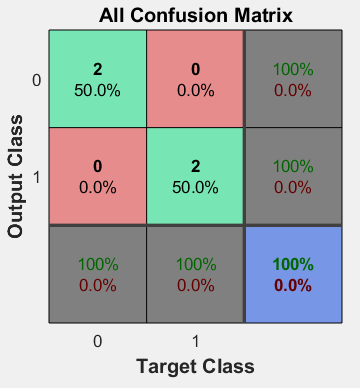
\includegraphics[width=0.4\textwidth]{pic2.png}
    \caption{分类数据上的混淆矩阵}
\end{figure}
\begin{figure}[htbp!]
    \centering
    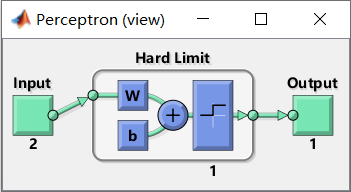
\includegraphics[width=0.5\textwidth]{pic3.png}
    \caption{神经网络参数结构}
\end{figure}
\newpage
通过可视化方法,可以将感知机分类的分割线绘制在图形中,得到如下的结果:
\begin{figure}[h]
    \centering
    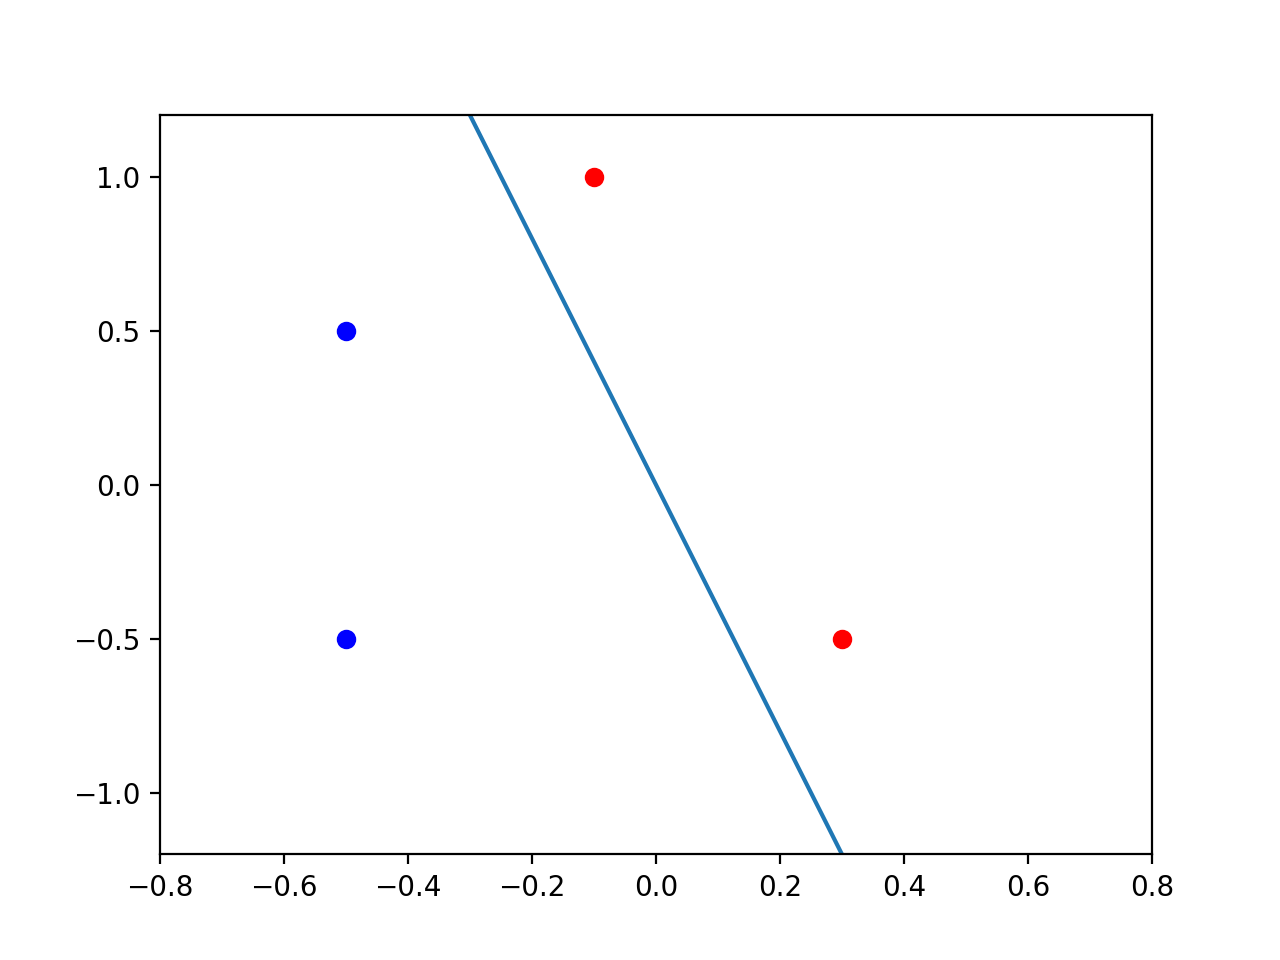
\includegraphics[width=1.0\textwidth]{pic4.png}
    \caption{分类情况}
\end{figure}
\end{document}
